\chapter{Summary}	


\begin{quote}
\emph{Well, I mean, yes idealism, yes the dignity of pure research, yes the pursuit of truth in all its forms, 
but there comes a point I'm afraid where you begin to suspect that the entire multidimensional infinity of 
the Universe is almost certainly being run by a bunch of maniacs.} \\
%And if it comes to a choice between spending 
%yet another ten million years finding that out, and on the other hand just taking the money and running, 
%then I for one could do with the exercise.
- Douglas Adams, \emph{The Hitchhiker's Guide to the Galaxy} (1979)
\end{quote}

In this thesis, measurements of the \bquark\to\squark electroweak penguin decay 
\BdToKpimm were made using the \lhcb detector at the \lhc. 
The world's best measurements of the dimuon forward-backward asymmetry \AFB
 and the fraction of \Kstarz longitudinal polarisation 
were presented along with the first measurement of the \kpi S-wave contribution to \BdToKpimm.

This thesis is based on data taken at \lhcb in 2011 during run 1 of the \lhc. 
The changing conditions of the data-taking environment from 2010 to 2011 required a re-development of the trigger for \BdToKstmm.
These results provided cross-checks in the first truly multi-variate trigger in \lhcb for data-taking during 2011 and beyond.

Two angular analyses of \BdToKstmm were presented. % in Chapter~\ref{chap:kstmm}.
The first angular analysis of \BdToKstmm using 0.38\invfb  of data measured \AFB and \FL in 6 bins of \qsq
providing the most precise measurements of these angular observables at the time.
The second angular analysis improved on the measurements of the first 
and also measured the angular observables \OS3, \OS9 and \OA9 using 1.0\invfb of data.
%These precision measurements of the \BdToKstmm angular observables has not only enabled 
%stringent constraints to be placed on the Wilson coefficients
% but also demanded consideration of the exact details of measurements of \BdToKstll decays.


The results obtained for the \BdToKstmm angular observables were combined with other measurements of \bsll and \btosgam decays to 
place the most precise constraints to date on the values of the Wilson coefficients \C{7}, \C{9} and \C{10} ~\cite{Altmannshofer:2012az}.
The measurements of the branching fraction of \Bsmm and \BdKstGam were used constrain the magnitudes of \C9 and \C{10} and the magnitude of \C{7} respectively.
The measurements of the inclusive branching fraction of $\B\to X_s \g$ and $\B\to X_s\ellell$~\cite{hfag:2012} along with the branching fraction of \BuToKmm were used to constrain combinations of the Wilson coefficients.
The measurements of the differential branching fraction, \AFB and \FL from \BdToKstmm presented in this thesis were used to constrain combinations of \C{7}, \C{9} and \C{10}.
The two dimensional contours obtained in Ref~\cite{Altmannshofer:2012az} for combinations of the real and imaginary parts of the Wilson coefficients are shown in Fig.~\ref{fig:summ:const}.
\begin{figure}[tbp]
\centering
\subfigure[Constraints on the real and imaginary parts of the left-handed Wilson coefficients]{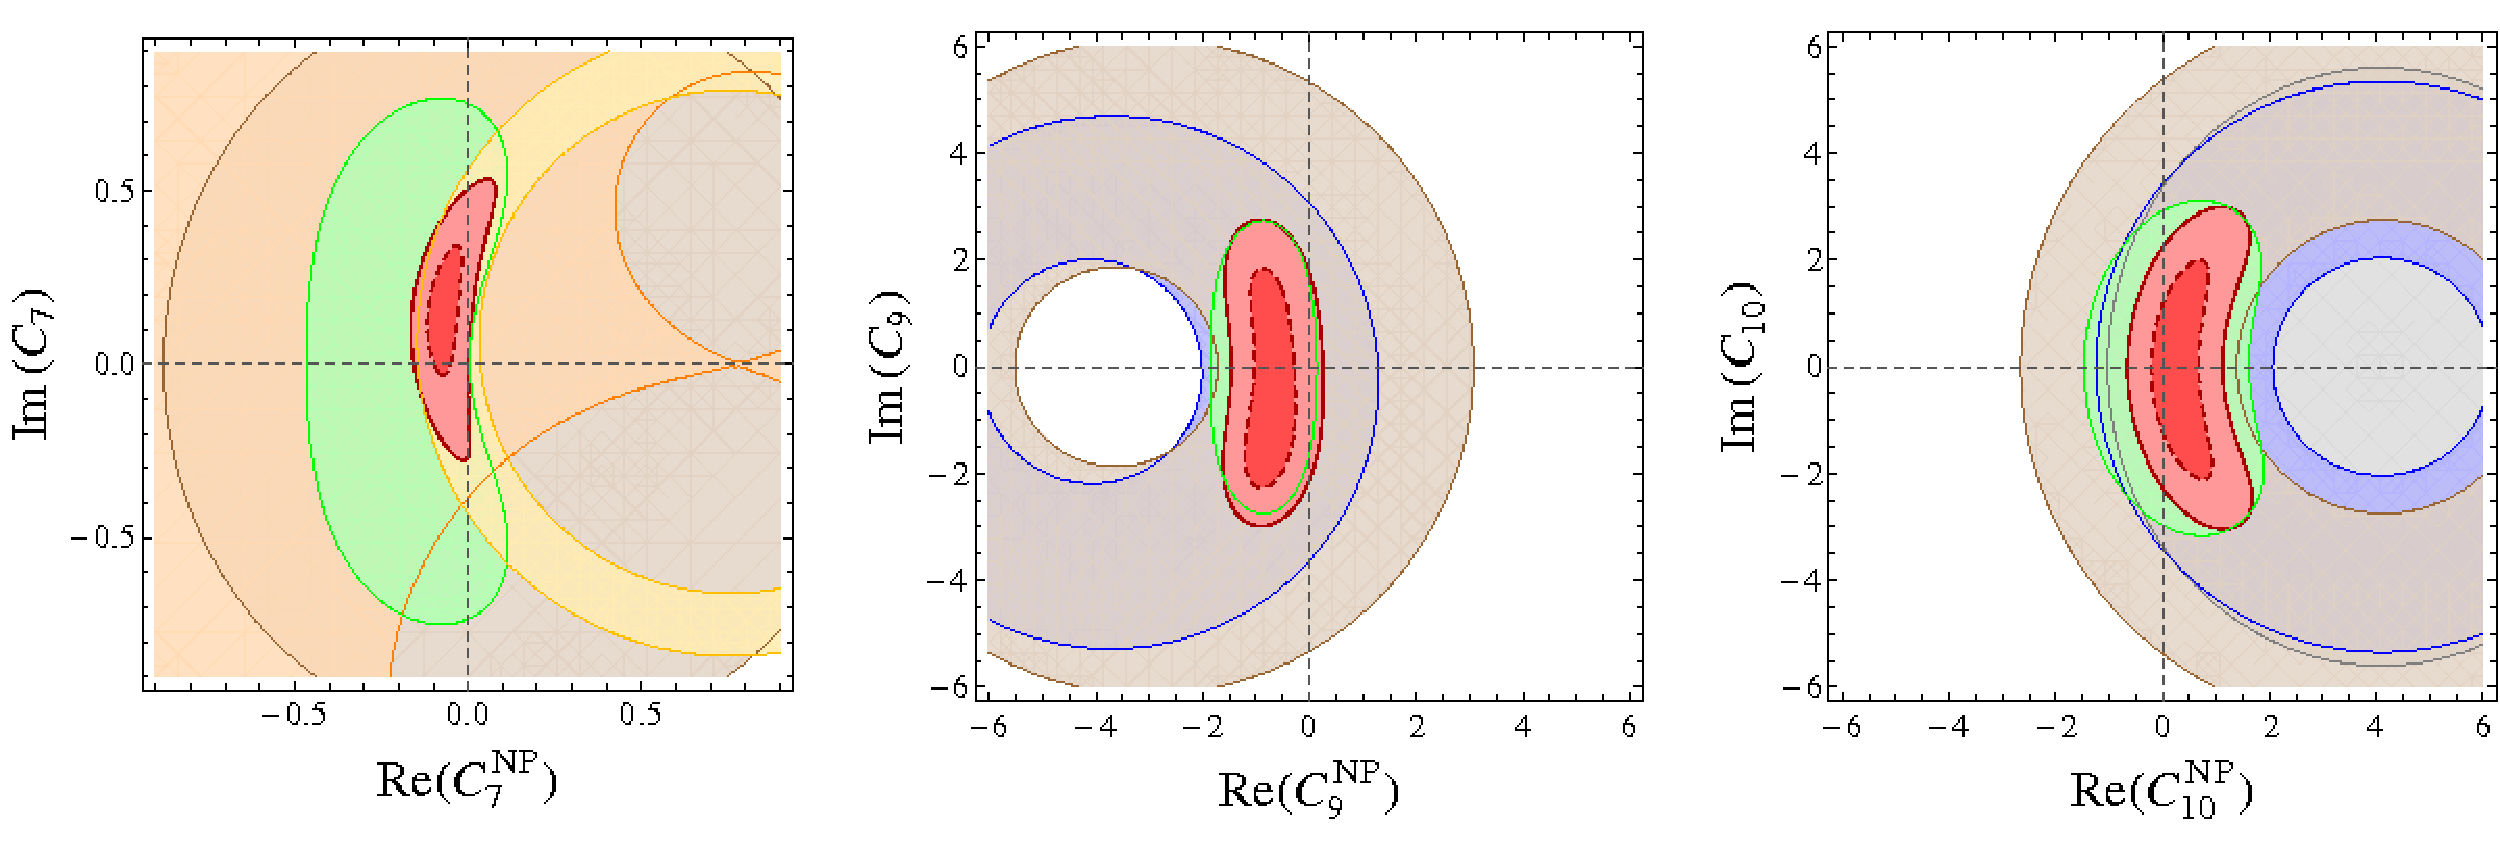
\includegraphics[width=0.88\columnwidth]{backmatter/figs/bandplotsSM_c.pdf}}
\subfigure[Constraints on the real and imaginary parts of the right-handed Wilson coefficients]{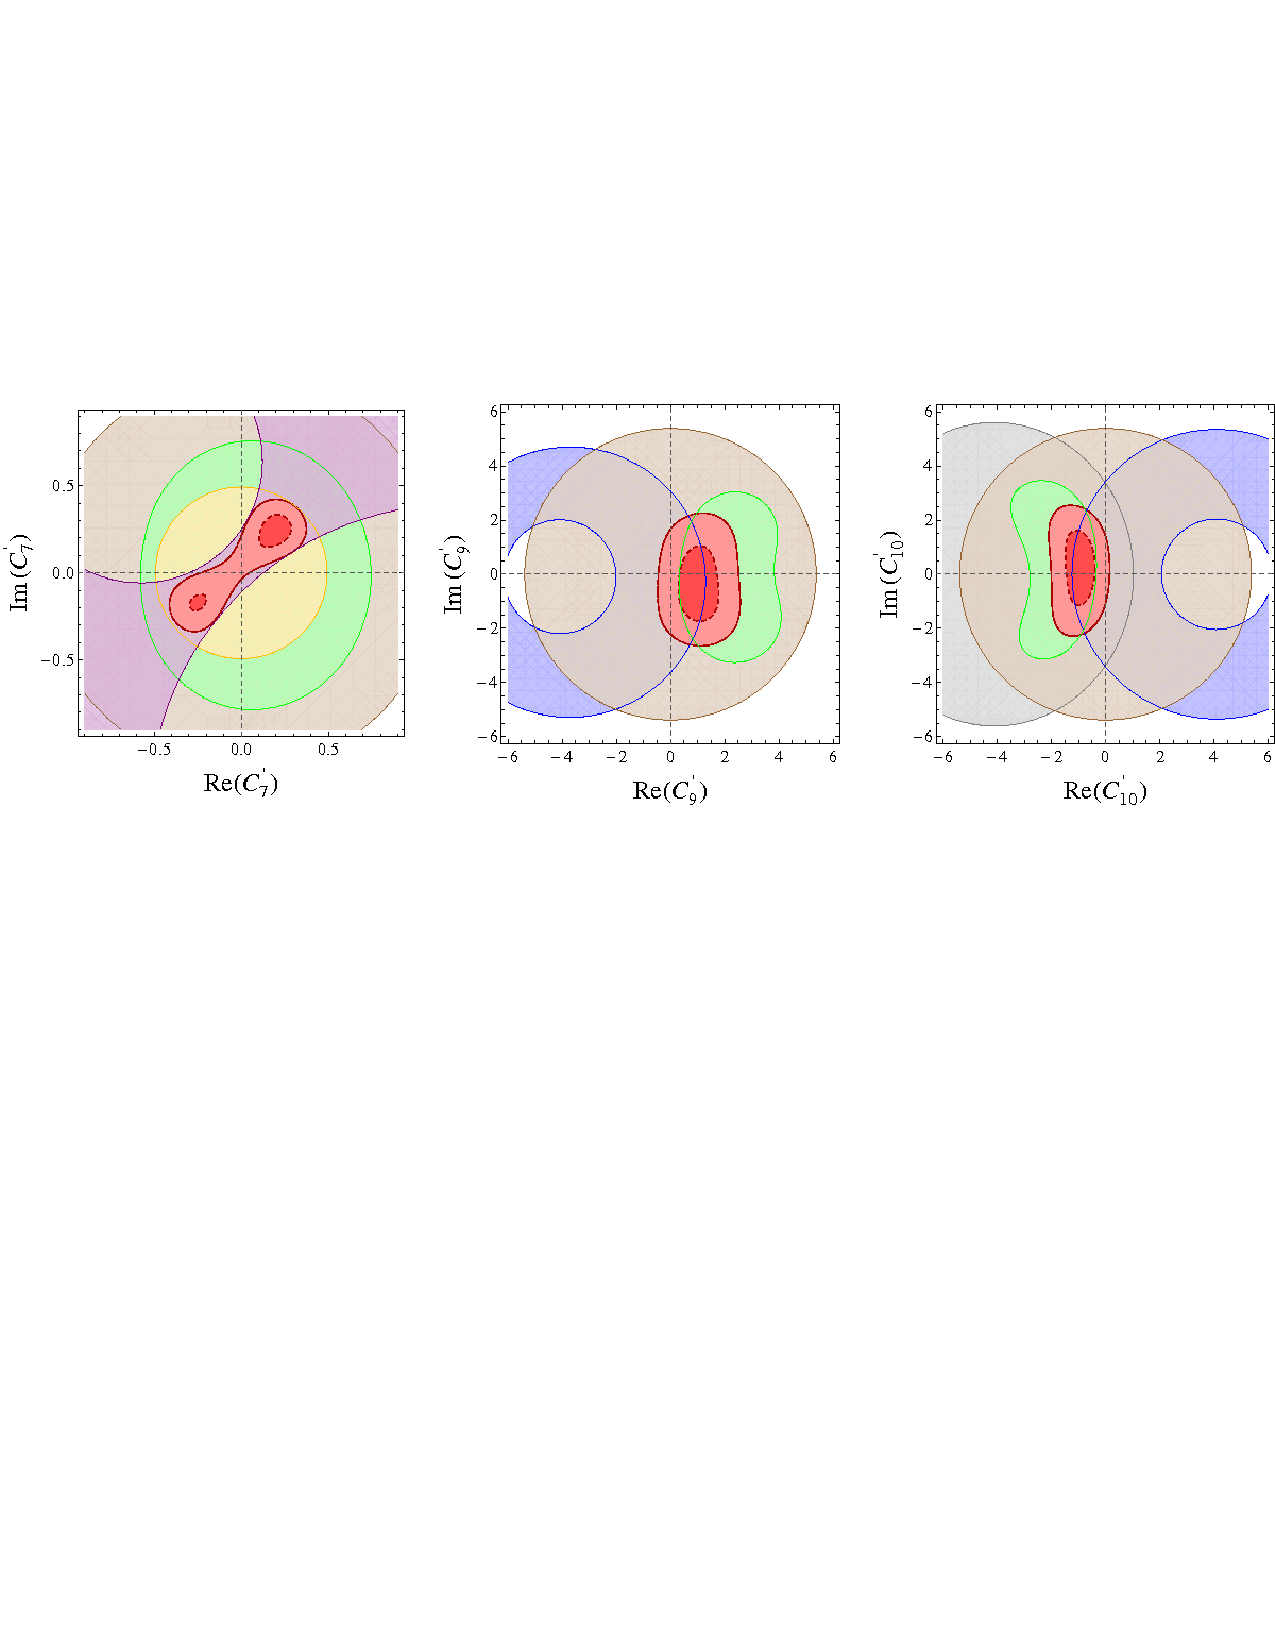
\includegraphics[width=0.88\columnwidth]{backmatter/figs/bandplotsRH_cc1.pdf}}
\subfigure[Constraints on the real part of the (\C{7,9,10} , \Cp{7,9,10} ) plane]{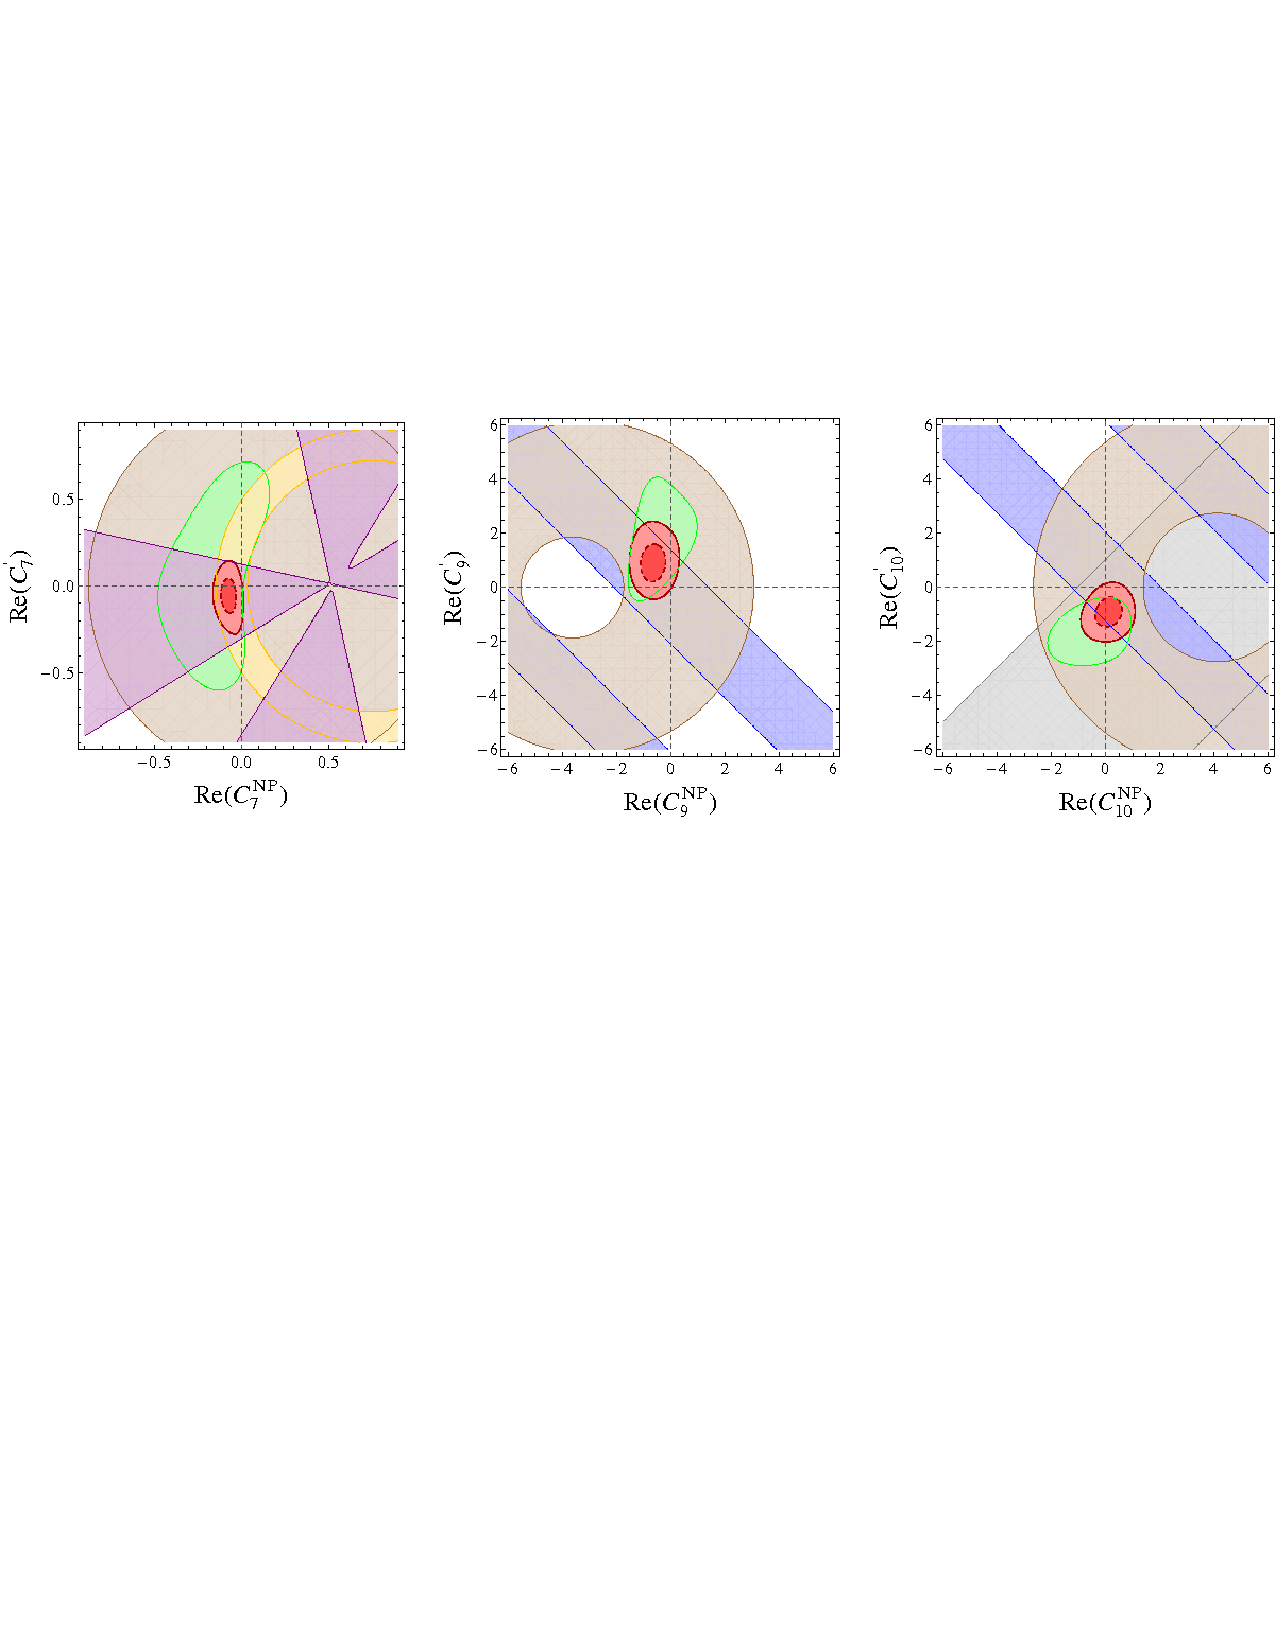
\includegraphics[width=0.88\columnwidth]{backmatter/figs/bandplotsRH_cc2.pdf}}
\caption{ Individual $2\sigma$ constraints on the unprimed Wilson coefficients from \BtoXsll (brown), \BR(\BtoXsg) (yellow), $A_CP$(\btosgam) (orange), \BdKstGam (purple), \BdToKstmm (green), \BuToKmm (blue) and \Bsmm (gray) as well as the combined 1 and $2\sigma$ constraints (pink and red respectively). Taken with permission from Ref.~\cite{Altmannshofer:2012az}.~\label{fig:summ:const}}
\end{figure}
These constraints are compatible with the SM prediction at the 2$\sigma$ level but it can be seen that the constraints placed on the imaginary parts of the Wilson coefficients are looser than the constraints placed on the real parts. 
%This comes from observables that are averaged over the \Bd and \Bdb CP eigenstates and implies that these limits do not exclude contributions from new particles that have a non-standard form of CP violation.

The measurement of observables in electroweak penguin decays are complementary to direct searches for specific signatures of new particles at \atlas and \cms at the \lhc. 
For example, the constraints on the Wilson coefficients can be converted into a limit on the mass of any new particle that contributes in \BdToKstmm of around $1\tev$~\cite{Altmannshofer:2012az}.
These limits can be compared to the limits on the mass of new particles of several hundred \gev from direct production, such as in Ref.~\cite{Chatrchyan:2013lya}.
The constraints obtained from electroweak penguin decays are model-independent to the level that they only assume that any new particles have similar couplings to the CKM elements in the SM.
wheras the limits from searches for the direct production of new particles place are dependent on the type of model used to produce the signature that is searched for.
% whearas the limits from the angular analysis of \BdToKstmm are only dependent on the model of the couplings between the new particles and the flavour sector.
A similar comparison can be made to the limits on the mass of dark matter particles from indirect scattering experiments~\cite{GeringerSameth:2011iw}. 

The inclusion of a \kpi S-wave in the angular distribution of \BdToKpill was shown to have an overall dilution effect on 
measurements of the \BdToKstll angular observables.
The toy studies presented here show significant bias on the angular observables from an S-wave contribution
of 7\% in the P-wave mass window for datasets of over 500 events.
In order to measure the size of this effect in data, the \kpi S-wave was measured using 1.0\invfb of data from \lhcb.
The integrated S-wave contribution between $0.64 < \psq < 1.00\gevgevcccc$ and between $1 < \qsq < 6\gevgevcccc$
is 
\begin{equation}
\FS = 0.083^{+0.057}_{-0.048}(\mathrm{stat.})^{+0.018}_{-0.050} (\mathrm{syst.})
 \, .
\end{equation}
The measurement shows that further investigation is required for any future angular analysis of \BdToKstmm.
The complete data recorded by \lhcb in 2011 and 2012 is expected to total 3.0\invfb. 
This gives 600 \BdToKstmm candidates between $1 < \qsq < 6\gevgevcccc$ which will result in a bias of $0.6\sigma$ in \FL and $0.3\sigma$ in \AFB if an S-wave of 7\% is ignored.

The next measurements of \BdToKstmm will be based on datasets of several thousand candidates from \lhcb and \cms. 
This will enable precision measurements of the angular observables in finer bins of \qsq in order 
to better determine the shape of \AFB at both low and high \qsq. 
%This is important as there are different theoretical approaches above and below the charmonium resonances.
Measurements of the \qsq value at which \AFB crosses zero will allow further tests of the SM predictions as
 theoretical predictions have reduced uncertainties from the form factors at this point.
%Beyond \BdToKstmm, further measurements of the difference between \bsll and \btodll penguins will test the ratio of CKM factors inherent in the decays and measurements of \btosmm and \btosee decays will test the difference in couplings between leptons for any asymmetry.

At the time of writing, the first run of the \lhc has finished and the machine has been shut down for 2 years in order to upgrade the accelerator. 
Although the first two years of data have resulted in the discovery of the Higgs, there are no obvious
hints of physics beyond the Standard Model in the measurements from the \lhc.
However, as direct searches yield few positive signs of physics beyond the SM, interest turns again to measuring the subtle effects in indirect searches.
The electroweak penguin decays of \bquark hadrons are already placing stringent constraints on the 
size of new physics couplings within the flavour sector. 
The datasets from the second run of the \lhc will enable precision measurements of both the \BdToKpill spectrum
and full angular analyses of \BdToKstmm. 

